\lettrine[lines=2, findent=3pt,nindent=0pt]{I}{n} this chapter we present a method to obtain a tight bound for the quantum Fisher information based on the expectation values of the initial prove state.

One of such criteria is
\be
  \mathcal{F}_{\text{Q}} [\rho,J_z] \geq \frac{\expect{J_x}^2}{\varian{J_y}}
\ee

\be
  \mathcal{B}_{\mathcal{F}}(w_1,w_2,...)
\ee

\begin{figure}
  \centering
  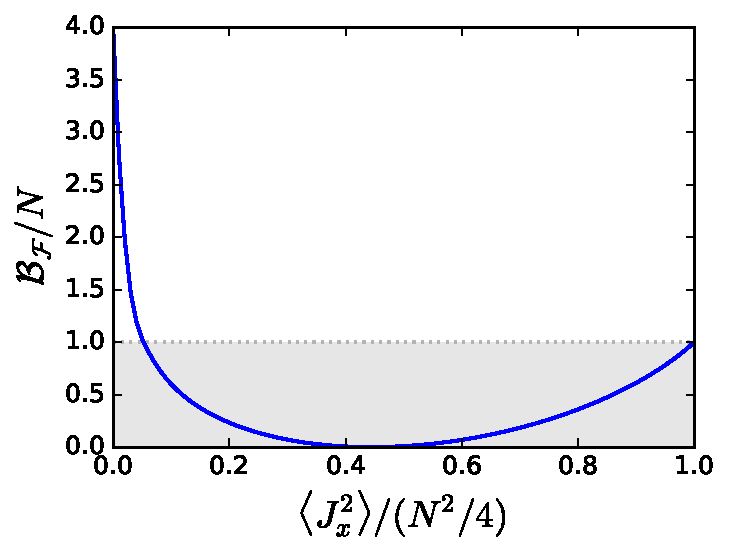
\includegraphics[scale=.65]{img/plots/LT_dicke_edge.pdf}
  \caption{[TODO: Correct the X-Label. It must be normalized by maxJx2]}
  \label{fig:vd-secuence-evo}
\end{figure}

\begin{figure}
  \centering
  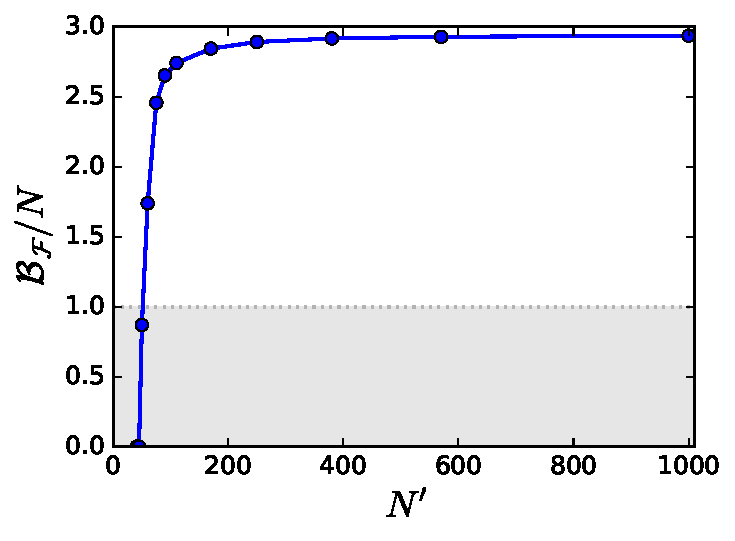
\includegraphics[scale=.65]{img/plots/LT_dicke_7900_asymp.pdf}
  \caption{Secuence of the evolution of an unpolarized Dicke state of 16 qubits for $\Theta=\{i\pi/6\}_{i=0}^4$. Bloch spheres representing the Hirusi distribution of the state, and below PDF of the $J_x$ POVM for each step of the secuence}
  \label{fig:vd-secuence-evo}
\end{figure}
